\chapter[Metodologia]{Metodologia}
\label{cap-metodologia}

Para cumprir com o objetivo fim de realizar uma Avaliação do Ecossistema de Startups de Tecnologia do Distrito Federal foi adotada a Metodologia criada por \citeonline{Cukier2015, Kon2014}, uma das primeiras contribuições do Grupo de Pesquisa em Empreendedorismo InovaSampa\footciteref{inovasampa}. 

A escolha se deu por recomendação do Orientador deste trabalho, Professor Paulo Meirelles, e por acreditar que ela fornece um bom caminho para obtermos uma visão geral e realista do atual estado do Ecossistema local por ter uma forte integração com empreendedores locais e já ter sido executada em três cidades do mundo: Tel-Aviv \citeonline{Kon2014}, São Paulo \citeonline{MonnaSantos2015} e Nova Iorque \citeonline{Cukier2016}. 

Também será a primeira vez que a metodologia em questão é aplicada por outra pessoa que não um de seus criadores, e sem uma orientação ou participação direta dos mesmos. Por esse motivo a maior parte das decisões tomadas e do conteúdo exposto nesse capitulo foram inferidos com base em artigos já publicados. 

Além da contribuição natural para o Ecossistema Empreendedor do Distrito Federal como um dos primeiros, se não o primeiro, trabalho acadêmico com foco exclusivo na capital ele também será a primeira aplicação da metodologia mencionada por uma pessoa que não um de seus criadores, esse contexto poderá fornecer feedbacks valiosos grupo de pesquisa InovaSampa sobre como se deu essa experiência durante três semestres e todas as adaptações que foram feitas afim de obter uma visão mais adequada com base nos dados disponíveis no nosso contexto. Este trabalho pode, inclusive, contribuir para a melhoria da metodologia e representar o primeiro passo para que ela também seja aplicada em outros Ecossistemas brasileiros além de São Paulo e Brasília.

\section{Trabalhos Relacionados}
\label{section:trabalhos_relacionados}

A Endeavor, por meio da Rede Global de Empreendedorismo, elabora o Índice de Cidades Empreendedores\footciteref{indiceglobaldoempreendedorismo} desde 2014 com o objetivo de ajudar ecossistemas locais a crescerem por meio da identificação de fatores que possam ser aprimorados de tal forma que o Índice pode ser um utilizado como uma espécie de guia para Governantes, Empreendedores engajados com o Ecossistema, Associações, etc. Atualmente ele conta com análise de 32 cidades, em sua maior parte capitais, e a tendência é que por meio da atuação dos Comitês Locais da Rede Global de Empreendedorismo o número de cidades expanda cada vez mais. O ranking de 2016 está disponível como Anexo \ref{anexo:indice_de_cidades_empreendedoras}.

A metologia tem como base sete pilares: ambiente regulatório, infraestrutura, mercado, acesso a capital, inovação, capital humano e cultura empreendedora. A maior dificuldade encontrada pelos pesquisadores fora a dificuldade em encontrar dados sistemáticos sobre o Ecossistema brasileiro, por exemplo motivo as principais fontes de dados são bases públicas mas nem sempre estão atualizadas, mas alguns estão sob domínio de terceiros, em sua maior parte entidades privadas, ou precisaram ser criados. 

Embora seja a análise mais completa já realizada sobre o Ecossistema Empreendedor de Brasília, o Índice de Cidades Empreendedoras não tem como foco o cenário de Startups e tem como uma forte base análises de dados quantitativos, mas é de altíssima importância para validar alguns dos pontos levantados por este trabalho.

\citeonline{Suresh2012} buscaram, por meio de um estudo qualitativo e revisões bibliográficas, mapear quais elementos encorajam as pessoas a seguirem o caminho do Empreendedorismo e encontraram oito fatores essenciais: Suporte Moral, desempenhado pelo circulo social dos empreendedores, Suporte Financeiro, seja por meio da família, governo, empréstimos ou investimentos, Suporte da Rede, no geral vindo de associações e comunidades, Suporte do Governo, Suporte de Tecnologia, desempenhado por centros de pesquisa e incubação, talentos disponíveis no mercado local, etc, Suporte do Mercado, Suporte Social, relacionado principalmente com a aceitação da falha da comunidade local e pelas ações da mídia, e Suporte do Ambiente, relacionado com recursos naturais e condições de clima.

\citeonline{Arnaud2009} e \citeonline{Ahmad2007} por meio da OECD definiram três grandes pilares para avaliar o Empreendedorismo em uma região. O primeiro, de Determinantes, é composto por indicadores Ambiente Regulatório, Cultura, Pesquisa \& Desenvolvimento e Tecnologia, Acesso à Financiamento, Capacidades Empreendedoras, Condições do Mercado. O segundo pilar, chamado de Performance Empreendedora, é composto por indicadores baseados nas empresas e nos empregos da região. O terceiro, de Impacto, estuda dados comos Criação de Empregos, Crescimento Econômico e Redução da Pobreza. No mesmo artigo são indicados diversas fontes e meios para se obter dados sobre esses indicadores.

\citeonline{Lemos2011} propôs uma metodologia para avaliação de Ecossistemas de Startups com o viés de apoiar o desenvolvimento de gestão estratética do Empreendedorismo dentro das universidades a partir do modelo de hélice tripla, que defende que para a atração de inovação e o desenvolvimento econômico de uma região cresçam é necessário uma forte integração entre Governo, Universidades e Indústria. Com base em outros autores ele introduz a importância de se adicionar os Empreendedores na equação e trás uma abordagem de análise qualitativa similar à deste trabalho para avaliação mas com foco na própria Academia.

\citeonline{Arruda2013} também realizaram um estudo muito similar à este trabalhao, analisando o Ecossistema Empreendedor Brasileiro de Startups por meio de uma abordagem mista de estudos Qualitativos, onde foram feitas 30 entrevistas com Empreendedores, Representantes de Instituições de Suporte, Investidores, Pesquisadores e Consultores de 5 estados brasileiros, e Quantitativos, com base nos fatores determinantes definidos por \citeonline{Arnaud2009}. 

Como resultados, obtiveram visões sobre o Modelo Regulatório Brasileiro, as nossas Condições de Mercado, o Acesso a Financiamento, a Criação e Difusão de Conhecimento, a Capacidade e a Cultura Empreendedora e as peculiaridades regionais do Brasil no que tange o Empreendedorismo e o mercado de Startups. O trabalho também lista em anexo todas as variáveis mapeadas para o trabalho e suas fontes, que foram de grande importância para este trabalho. Nas recomendações de trabalho futuro mencionam a dificuldade em conversar sobre experiências de fracasso com os Empreendedores Brasileiros, em especial com aqueles que ainda não alcançaram o sucesso, talvez esse problema se repita no contexto do Distrito Federal.

\citeonline{Sipola2013} mapearam os atores Consumidores, Inovadores, Empreendedores, Capital de Risco, Mercados de Saída(venda) e Indústrias como peças chaves para um Ecossistema de Startups. 

Os Inovadores são importantes por serem os atores responsáveis por mesclar novas e velhas tecnologias com o objetivo de criar algo novo que seja melhor, mais rápido e mais barato. Empreendedores são aqueles que transformam inovações em produtos em financeiramente viáveis e escaláveis. As Indústrias são responsáveis por permitirem que os melhores produtos sejam produzidos e distribuídos em larga escala. Sem os Mecânismos de Saída não seria possível atrair Capital de Risco e manter o ciclo de expansão e crescimento de negócios existentes e maduros e investimentos em novos negócios funcionando. E, por fim, todo esse ciclo tem como seu ponto central o Consumidor, sem ele, ou ela, o Empreendedorismo e as Inovações perderiam seus propósitos.

\citeonline{Kutt2013}, por meio de uma análise quantitativa de diversas bases de dados locais e globais fez uma comparação do Ecossistema de Startups da Estônia em um contexto internacional, comparando-o como Finlândia, Taiwan, Israel, Coreia e Singapura. O autor também fez um estudo por meio da análise de dados de redes sociais para obter uma visualização das estruturas sociais do Ecossistema da Estônia e identificar como os atores se conectam entre si.

\citeonline{Hermann2015} por meio do ``The Global Startup Ecosystem Ranking'' e da Compass realizaram um estudo dos principais Ecossistemas de Startups do mundo com base em seis pilares principais: Performance, Financiamento, Alcance de Mercado, Talento, Experiência em Startups e Índice de Crescimento. O ranking de 2015 está disponível como Anexo II, cada coluna representa um pilar e os valores numéricos em cada uma delas representam a posição de cada Ecossistema no pilar correspondente. 

Esse é um dos trabalhos disponíveis mais extensos que já foram realizados no contexto de Ecossistemas de Startups no mundo, cerca de 11 mil participantes de 40 Ecossitemas participaram da pesquisa por meio de questionários, mais de 200 especialistas de 25 países foram entrevistados e aproximadamente 35 mil empresas de tecnologia tiveram seus dados estudados pela Compass, também foram avaliadas diversas bases de dados públicas. Ele também teve uma grande contribuição na metodologia utilizada como base para este trabalho, criada por \citeonline{Cukier2015, Kon2014}, mas, mas como explorado em \ref{subsection:vantagens_e_desvantagens} não será de muita utilidade no contexto do Distrito Federal por ter como referência a cidade de São Paulo.

\citeonline{Kon2014}, em um dos primeiros artigos do grupo InovaSampa, relatam que foram encontrados poucos trabalhos que criam um arcabouço conceitual ou visões de Ecossistemas de Startups, mas mencionam \citeonline{Chorev2006} por terem mapeado alguns fatores críticos para o sucesso de uma Startup com base nas visões de 9 Empreendedores, divididos em grupos de acordo com a maturidade de suas Startups, e 3 Investidores. Os fatores de sucesso estão representados na Figura \ref{figure:success_or_failure_factors_model}.

\begin{figure}[!htb]
\centering
\includegraphics[width=11cm,angle=0]{figuras/success_or_failure_factors_model}
\caption{Fatores que influenciam o sucesso de uma Startup criado por \citeonline{Chorev2006}}
\label{figure:success_or_failure_factors_model}
\end{figure}

Kon também menciona o trabalho de \citeonline{Frenkel2014}, por criar um mapa visual de um Ecossistema de Inovação muito similar ao do trabalho realizado pelo InovaSampa porém obtendo os dados com a realização de um workshop e não diversas entrevistas individuais, e o modelo para avaliação de Inovação criado por \citeonline{Belitz2011} representado pela Figura \ref{figure:innovation_model}. 

\begin{figure}[!htb]
\centering
\includegraphics[width=11cm,angle=0]{figuras/innovation_model}
\caption{Modelo de Avaliação de Inovação por \citeonline{Belitz2011}}
\label{figure:innovation_model}
\end{figure}

Por ter sido uma imagem extraída do artigo citado e criada pelos autores mencionados, é importante ressaltar que a letra ``D'' representa Demanda, a letra ``E'' representa Educação, as letras ``R\&D'' representam Pesquisa e Desenvolvimento, a letra ``N'' representa ``Networking'', a letra ``I'' representa Implementação, as letras ``S\&T'' representam Ciência e Tecnologia e as letras ``SC'' representam Capital Social. \citeonline{Kon2014} enfatiza que muitos desses fatores estão presentes em seu arcabouço conceitual de um Ecossistema de Startups, com a diferença em que seu estudo foram explorados o relacionamento entre esses fatores ao invés de trata-los de forma isolada. \citeonline{Stam2015} também criou um arcabouço conceitual de um Ecossistema de Startups, parte de seu trabalho está representado na Figura \ref{figure:elements_of_an_ecosystem}.

\begin{figure}[!htb]
\centering
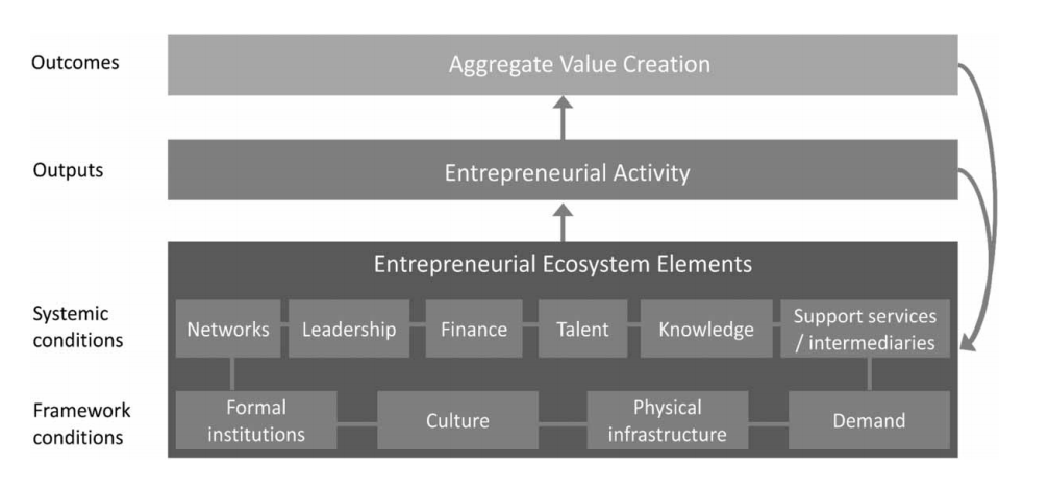
\includegraphics[width=11cm,angle=0]{figuras/elements_of_an_ecosystem}
\caption{Elementos de um Ecossistema por \citeonline{Stam2015}}
\label{figure:elements_of_an_ecosystem}
\end{figure}

\section{A Metodologia do InovaSampa}
\label{section:metodologia_do_inovasampa}

\subsection{Desvantagens e Vantagens}
\label{subsection:vantagens_e_desvantagens}

Até a publicação deste trabalho as três cidades que foram objetos de estudo do InovaSampa, e que contribuiram para a construção dessa Metodologia, são conhecidas globalmente como grandes centros empreendedores e dispõem de uma vasta quantidade de dados de pesquisas locais, regionais e globais disponíveis, o que não condiz com a realidade de Ecossistemas menores e menos estruturados, como o de Brasília. Isso torna alguns dos fatores ou medidas sugeridos fora de contexto com o que temos disponível, visto que infelizmente ainda não existe produção de dados sistemáticos sobre os diversos ambientes empreendedores menores e o acesso à informações confiáveis e atualizados é um problema.

%Para contornar esse problema, e trazer melhorias à Metodologia para que ela possa ser melhor utilizada no contexto de outras cidades brasileiras que também carecem de dados e querem conhecer e desenvolver seus Ecossistemas, alguns fatores foram excluídos ou adaptados para se adaptarem às informações disponíveis. Tudo está descrito na sessão \ref{subsection:fatores_que_formam_um_ecossistema}.

A maior vantagem da Metodologia proposta se dá por ter, como sua maior base, dados obtidos a partir das visões daqueles que melhor o entendem e lidam com o Ecossistema de Startups local - os próprios empreendedores. Ao dar uma maior prioridade a essa abordagem ao invés de uma análise puramente quantitativa com base em dados puramente estatísticos torna-se possível obter uma visualização mais realista e próxima de quais são as características mais fortes e fracas do Ecossistema em estudo como um todo.

\subsection{Técnicas Utilizadas}
\label{subsection:tecnicas_utilizadas}

Toda a metodologia foi construida com base nas técnicas de Pesquisa Qualitativa e na Teoria Fundamentada em Dados por oferecerem a possibilidade de obter dados a partir das visões daqueles que melhor o entendem e lidam com o Ecossistema de Startups local e seus pontos fortes e fracos todos os dias - os próprios empreendedores - por meio de entrevistas, dessa forma é possível valorizar e obter respostas a partir de suas experiências individuais.

\citeonline{Maxwell2013} define uma Pesquisa Qualitativa como uma pesquisa que tem como objetivo ajudar o Pesquisador a entender as perspectivas das pessoas estudadas - o mundo pelo ponto de vista de quem faz parte do objeto de estudo e não do ponto de vista do Pesquisador, como essas perspectivas moldam e influenciam o contexto estudado e como todos esses fatores se envolvem com os fenômenos e relacionamentos em estudo. \citeonline{Merriam1991} diz que o processo e o conhecimento obtido durante o estudo são mais importantes do que os resultados finais. Isso é possível graças a uma abordagem flexível que tem como base uma abordagem visual, falada ou textual, ao invés de estatística como trabalhado pela Pesquisa Quantitativa. Maxwell diz que o Pesquisador que opta por trabalhar com a Pesquisa Qualitativa quer enxergar o mundo através de pessoas, situações, eventos e processos que os conectam.

O referido autor também diz que as atividades de coletas e análise de dados, desenvolvimento de fundamentações teóricas, elaborações de questões de pesquisa e identificações e validações de conceitos geralmente evoluem juntos durante uma abordagem qualitativa e que um bom projeto possui componentes que se relacionam de forma harmônica. Alguns dos pontos fortes de uma Pesquisa Qualitativa de acordo com Maxwell estão representados pela Tabela \ref{table:objetivos_intelectuais_segundo_maxwell} e alguns dos objetivos pela Tabela \ref{table:pontos_fortes_segundo_maxwell}.

\begin{table}[!htb]
	\centering
	\begin{tabular}{ | p{3cm} | p{12cm} | }
		\hline
		1 & Entender o significado, de acordo com os participantes do estudo, dos eventos, situações, experiências e ações em que eles se envolvem ou engajam. \\ \hline
		2 & Entender os contextos particulares em que os participantes do estudo atuam e como esses contextos impactam em suas decisões. \\ \hline
		3 & Entender o processo o qual eventos e ações acontecem. \\ \hline
		4 & Identificar fenômenos e influências não previstos gerando novas teorias fundamentadas em dados sobre o objeto estudado. \\ \hline
	\end{tabular}
	\caption{Alguns dos pontos fortes de uma Pesquisa Qualitativa, por \cite{Maxwell2013}}
	\label{table:objetivos_intelectuais_segundo_maxwell}
\end{table}

\begin{table}[!htb]
	\centering
	\begin{tabular}{ | p{3cm} | p{12cm} | }
		\hline
		1 & Gerar teorias e resultados que sejam válidos e compreensíveis tanto para as pessoas que estão sendo estudadas como também para outras pessoas, que possam ou não ser pesquisadores. \\ \hline
		2 & Melhorar práticas, programas ou políticas existentes ao invés de simplesmente avalia-las, por esse motivo é importante entender os processos e contextos específicos dessas ações e como elas são vistas pelos participantes da pesquisa. \\ \hline
		3 & Engajar-se em ações participativas, colaborativas ou com foco na comunidade junto com os participates do estudo. \\ \hline
	\end{tabular}
	\caption{Alguns dos objetivos de uma Pesquisa Qualitativa, por \cite{Maxwell2013}}
	\label{table:pontos_fortes_segundo_maxwell}
\end{table}

Em relação ao significado da Teoria Fundamentada em Dados \citeonline{Glaser1999} diz que se trata de uma série de conhecimentos que são desenvolvidos de forma indutiva durante o estudo e com uma forte integração com os dados coletados, a teoria que será criada será altamente dependente e fundamentada nesses dados, diferente de uma teoria que é construída de forma conceitual e depois validada.

\subsection{Fatores que formam um Ecossistema}
\label{subsection:fatores_que_formam_um_ecossistema}

Após vasta pesquisa bibliográfica e entrevistas com mais de 50 pessoas chaves para os Ecossistemas de Tel-Aviv e São Paulo foram definidos cerca de 21 fatores que os compõem e fazem parte do Arcabouço Teórico de um Ecossistema, descrito na subseção \ref{subsection:arcabouco_conceitual_e_modelo}. Com o objetivo de classifica-los entre níveis para facilitar as comparações e o cálculo final da maturidade do Ecossistema foram definidas as seguintes métricas para cada um dos fatores representados na Tabela \ref{table:metricas_de_classificacao_dos_fatores}, vale ressaltar que os fatores que contém o símbolo \"*\" antes de seu nome são os fatores essenciais, os restantes são os fatores derivados.

\begin{table}[!htb]
\centering
\begin{tabular}{llll}
Fator                                                      &     L1     &     L2     &     L3      \\
Estratégias de Saída*                                      &     00     &     01     &    >=2      \\
Mercado Global*                                            &    <10\%   &   10-40\%  &    >40\%    \\
Empreendedorismo nas Universidades*                        &    <02\%   &   02-10\%  &    >10\%    \\
Qualidade de Mentores                                      &    <10\%   &   10-50\%  &    >50\%    \\
Burocracia                                                 &    >40\%   &   10-40\%  &    <10\%    \\
Gastos com impostos                                        &    >50\%   &   30-50\%  &    <30\%    \\
Qualidade das Aceleradoras                                 &    <10\%   &   10-50\%  &    >50\%    \\
Acesso à investimento em US\$ por ano                      &    <200M   &   200M-1B  &    >1B      \\
Qualidade do Capital Humano                                &    >20th   &   15-20th  &    <15th    \\
Valores Culturais para o Empreendedorismo*                 &    <0.5    &   0.5-0.75 &    >0.75    \\
Processos de Transferência de Tecnologia                   &    <4.0    &   4.0-5.0  &    >5.0     \\
Conhecimento das Metodologias                              &    20\%    &   20-60\%  &    >60\%    \\
Atores da Mídia com foco no Empreendedorismo               &    <03     &   03-05    &    > 05     \\
Eventos relacionados à Startups*                           &   monthly  &   weekly   &    daily    \\
Dados do Ecossistema e Pesquisas*                          &    nada    & parcial    & disponíveis \\
Gerações do Ecossistema*                                   &     00     &    0.1     &    02       \\
Número de Startups*                                        &    <200    &   200-1k   &    >1k      \\
Acesso à investimento em quantidade de negócios/ano        &    <50     &   50-300   &    >300     \\
Acesso à investimento anjo em quantidade/ano*              &    <05     &   05-50    &    >50      \\
Incubadoras e Parques Tecnológicos                         &     01     &    02-05   &    >5       \\
Presença de Empresas de Alta Tecnologia*                   &    <02     &   02-10    &    >10      \\
Influência de Empresas já estabelecidas                    &    <02     &   02-10    &    >10      \\
\end{tabular}
\caption{Métricas de classificação dos Fatores que compõem um Ecossistema}
\label{table:metricas_de_classificacao_dos_fatores}
\end{table}

Uma descrição de cada um dos fatores citados está disponível no Apêndice \ref{apendices:fatores_de_um_ecossistema}.

\subsection{Versão Enxuta do Modelo de Avaliação}
\label{subsection:versao_enxuta_do_modelo_de_avaliacao}

Também foi desenvolvido uma versão mais enxuta do Modelo, com foco em apenas oito fatores ao invés de 21. Os parâmetros utilizados estão representados na Figura \ref{figure:short_version_maturity_model} e a importância de cada um dos fatores na Figura \ref{figure:metrics_importance}.

\begin{figure}[!htb]
\centering
\includegraphics[width=11cm,angle=0]{figuras/short_version_maturity_model}
\caption{Parâmetros utilizados pela versão enxuta do Modelo de Maturidade por \citeonline{Cukier2016}}
\label{figure:short_version_maturity_model}
\end{figure}

\begin{figure}[!htb]
\centering
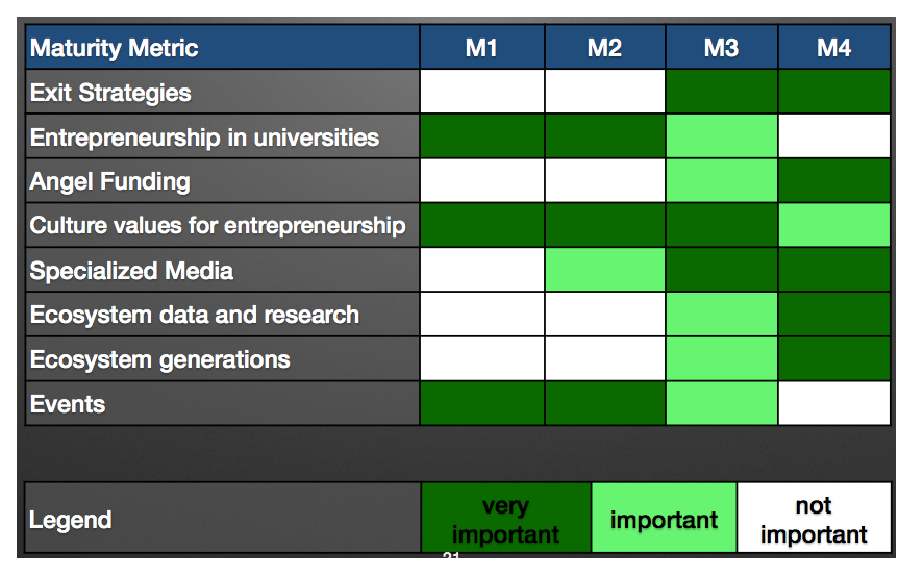
\includegraphics[width=11cm,angle=0]{figuras/metrics_importance}
\caption{Importância das Métricas citadas para cada um dos níveis de maturidade por \citeonline{Cukier2016}}
\label{figure:metrics_importance}
\end{figure}

\subsection{O arcabouço conceitual e o Mapa de um Ecossistema}
\label{subsection:arcabouco_conceitual_e_modelo}

Com base nesses mesmos fatores descritos na subseção \ref{subsection:fatores_que_formam_um_ecossistema} e na relevância de cada um deles de acordo com a visão das pessoas que compõem o próprio Ecossistema e nas informações disponibilizadas por outras pesquisadores ou bases de dados foi elaborado um arcabouço conceitual de um Ecossistema, representado pela Figura \ref{figure:arcabouco_teorico_de_um_ecossistema}. Nas Figuras \ref{figure:mapa_conceitual_tel_aviv}, \ref{figure:mapa_conceitual_sao_paulo} o Mapa do Ecossistema de São Paulo, ambos tendo como base o mesmo arcabouço conceitual. Os três Mapas Conceituais estão disponíveis no Anexo \ref{anexo:mapas_concentuais_do_inovasampa}.

\subsection{Os níveis de maturidade de um Ecossistema}
\label{subsection:niveis_de_maturidade_de_um_ecossistema}

Além de elaborar o mapa do ecossistema a Metodologia tem como um dos seus objetivos classificar Ecossistemas entre quatro diferentes níveis de maturidade. Os níveis são os seguintes:

\begin{description}
  \item [Nascente (M1):] quando há um Ecossistema com algumas Startups presentes no mercado, alguns investimentos concretizados e algumas iniciativas com o objetivo de estimular ou fomentar o Ecossistema sendo realizadas mas não há reconhecimento ou as Startups não possuem representatividade nos índices de geração de emprego e renda da região.

  \item [Crescente (M2):] quando há algumas Startups estabelecidas como empresas sólidas e o Ecossistema como um todo possui representatividade notável na economia regional e nos índices de empregos. Para se enquadrar como Crescente todos fatores essenciais e cerca de 30\% dos fatores derivados deverão ser classificadas como nível L2.

  \item [Maduro (M3):] quando existem algumas centenas de Startups em atividade, sendo algumas reconhecidas internacionalmente e com negócios realizados globalmente, um histórico relevante de investimentos concretizados dentro do Ecossistema e pelo menos uma geração de empreendedores bem sucedidos que se tornaram líderes, mentores, referências e investidores-anjo para os novos empreendedores, ajudando-os a crescer. Além dessas características, para ser considerado como um Ecossistema Maduro, todos os fatores essenciais e pelo menos 50\% dos fatores derivados devem ser classificadas como nível L2 e, no mínimo, 30\% de todos os fatores devem estar enquadrados no nível L3.

  \item [Sustentável (M4):] quando o número de Startups em atividade e de aquisições e/ou investimentos dentro do Ecossistema ultrapassam a casa dos milhares, há no mínimo duas gerações de empreendedores bem sucedidos que iniciaram suas carreiras com Startups de tecnologia presentes, uma rede de empreendedores comprometidos com o desenvolvimento do Ecossistema à longo prazo, um ambiente inclusivo com muitos eventos envolvendo temáticas que fomentem a cultura empreendedora e o mercado local e a presença de uma alta quantidade de profissionais de alta qualidade técnica. Para possuir esse estágio de maturidade, todos os fatores essenciais devem ser classificados como nível L3 e pelos menos 80\% dos fatores derivados também como nível L3.
\end{description}

\section{Aplicação da Metodologia e Protocolo}
\label{section:aplicacao_da_metodologia}

A aplicação da Metodologia foi dividida em três etapas:

\begin{enumerate}
  \item Entrevistas e Observações
  \item Codificação dos Dados
  \item Análises e Conclusões
\end{enumerate}

A primeira, de Entrevistas e Observações, se deu por meio da observação de diversos eventos que movimentam o Ecossistema de Startups do Distrito Federal e das pessoas que o compõem e por meio de entrevistas individuais com pessoas atuantes no Ecossistema com objetivo de entender seu contexto pessoal e profissional, bem como suas visões sobre a realidade e as dinâmicas do Ecossistema como um todo, quais os seus pontos fortes e fracos, seus maiores problemas, como diversas instituições e pessoas interagem entre si afim de fomenta-lo e quais ações poderiam ser tomadas afim de melhora-lo.

Com a Codificação dos Dados todas as informações levantadas pela primeira etapa foram catalogadas em tabelas com o objetivo de se tornarem referências para as etapas de Análises e Conclusões e futuras pesquisas bem como documentar todo o processo que foi realizado. 

Com as Análises dos dados e sua adequação nos fatores pré-definidos será possível mensurar a maturidade do Ecossistema com o objetivo de gerar as Conclusões da pesquisa, que se concentrarão em explicitar o atual estágio do Ecossistema de acordo com a Metodologia utilizada, em realizar comparações com outros Ecossistemas e identificar uma série de ações que podem ser tomadas para aprimorar determinados pontos.

\subsection{Questões de Pesquisa}
\label{subsection:questoes_de_pesquisa}

\citeonline{Maxwell2013} define Questões de Pesquisa como o que, especificamente, o Pesquisador espera entender com o desenvolvimento da pesquisa. Com base nessa premissa, as questões à serem respondidas sobre o Ecossistema de Startups do Distrito Federal são as seguintes:

\begin{itemize}
  \item Questão de Pesquisa 1: Quais são as características socioculturais de Brasília que promovem ou inibem o espirito empreendedor?
  \item Questão de Pesquisa 2: Quais são os mecânismos institucionais de Brasília que promovem ou dificultam o Empreendedorismo?
  \item Questão de Pesquisa 3: Quais são os mecânismos educacionais de Brasília que promovem o Empreendedorismo?
  \item Questão de Pesquisa 4: Como os fatores tecnológicos influenciam o sucesso ou fracasso das Startups de Brasília? Qual o papel executado pela comunidade e pelo Software Livre?
  \item Questão de Pesquisa 5: Qual a relação do empreendedor de Brasília com as opções de investimento disponíveis e como elas influenciam o Ecossistema?
  \item Questão de Pesquisa 6: Quais ações devem ser tomadas no Ecossistema de Brasília para que ele cresça?
\end{itemize}

Vale ressaltar que muitas delas são exatamente como as definidas no mapeamento de Tel-Aviv realizado por \citeonline{Kon2014} e de São Paulo por \citeonline{MonnaSantos2015}.

\subsection{Escolha dos Entrevistados}
\label{subsection:escolha_dos_entrevistados}

É de extrema importância que os entrevistados sejam atuantes e bem conectados com o Ecossistema de Startups do Distrito Federal como um todo e, em sua maior parte, Empreendedores mas Professores, Servidores e Agentes Públicos, Investidores, Representantes de Incubadoras e Aceleradoras e Estudantes também serão consultados. A meta é que sejam entrevistados cerca de 20 pessoas destes grupos.

Assim como sugerido pelos criadores da Metodologia, para a escolha dos Entrevistados fora aplicada a metodologia bola de neve. Primeiramente foram definidos algumas pessoas com alto histórico de contribuição e participação no Ecossistema e que faziam parte da rede de contatos das pessoas envolvidas com a Pesquisa e foram pedidos recomendações de quais pessoas deveriam fazer parte desta pesquisa e, se possível, solicitado uma introdução entre essas pessoas. Ao fim de cada entrevista esse processo também será repetido. 

\subsection{Condução das Entrevistas}
\label{subsection:conducao_das_entrevistas}

Todas as entrevistas devem ser realizadas, preferencialmente, no ambiente profissional dos Empreendedores de forma a mantê-los à vontade. Caso não seja possível, ela poderá ser conduzida em ambiente escolhido pelo empreendedor, como bibliotecas, cafeterias ou eventos e apenas em último caso de forma remota. Elas também serão gravadas em aúdio caso haja consentimento do empreendedor afim de facilitar a fase de Codificação dos Dados.

Elas não devem ser muito longas, preferencialmente não sendo extendidas por mais de uma hora e meia. Para guiar o Entrevistador foram estabelecidas uma série de Perguntas que devem ser realizadas aos Entrevistados com o objetivo de obter respostas que respondam às Questões de Pesquisa estabelecidas em \ref{subsection:questoes_de_pesquisa} e que nos forneçam uma visão geral do Ecossistema. 

Não necessariamente as entrevistas devem seguir de forma rígida todas as perguntas definidas no roteiro, o entrevistador poderá ter liberdade de conduzi-la como bem entender. Como a entrevista será conduzida ou a linguagem utilizada não é de grande importância, desde que a maior parte das questões sejam respondidas, mesmo que de forma indireta. Há a possibilidade de que o próprio entrevistado responda algumas delas durante outras perguntas. 

Todas as perguntas e o roteiro sugerido estão disponíveis no Apêndice \ref{apendices:perguntas_das_entrevistas}.

\subsection{Transcrição, Codificação e Interpretação dos Dados}
\label{subsection:codificacao_e_interpretacao_dos_dados}

Após a realização de cada Entrevista a transcrição e codificação das entrevistas será feita utilizando o software MAXQDA, a escolha por esse software se deu por recomendação dos próprios criadores da metodologia e com base em uma pesquisa sobre as opções disponíveis.